%!TEX root =  ../main.tex
\renewcommand{\columnseprule}{1.5pt}
\begin{multicols*}{2}
\rule[0.5\baselineskip]{0.4\textwidth}{1pt}
\noindent
\LabSection{Through the Looking Glass}\label{sec0104p}
\begin{exercises}{sec0104p}
\lab[0104LabTable]In the four, blank squares below, fill in the correct sign (positive or negative) 
of the answer.
Take a number of the sign given on the left, to a power of the kind given above.  For example, 
the top-left square is asking for the \emph{sign} of a positive number to an even power (e.g. $31^{60}$).  This means the top-left square is ``+''.

\noindent
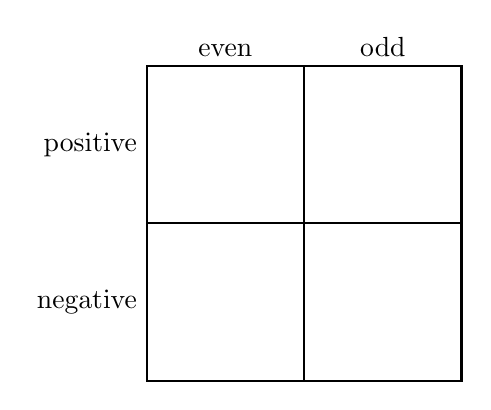
\begin{tikzpicture}
	\draw [thick,-] (0,0) -- (4,0) -- (4,4) -- (0,4) -- cycle;
	\draw [thick,-] (2,0) -- (2,4);
	\draw [thick,-] (0,2) -- (4,2);
	\draw (0,1) node[anchor=east] {negative};
	\draw (0,3) node[anchor=east] {positive};
	\draw (1,4) node[anchor=south] {even};
	\draw (3,4) node[anchor=south] {odd};
\end{tikzpicture}

\lab[0104LabSquared] Plot the graph of $y=x^2$ without using a graphing calculator.  
Leave $x$ 1:1, but scale the $y$-values 1:10.

\noindent
\begin{centering}
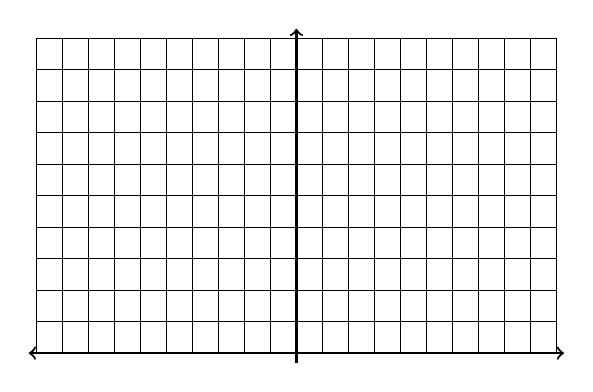
\begin{tikzpicture}[xscale=0.33,yscale=0.04]
	\draw [thick, <->] (-10.3,0) -- (10.3,0);
	\draw [thick, ->] (0,-3) -- (0,103);
	\draw [thin,ystep=10] (-10,0) grid (10,100);
\end{tikzpicture}
\end{centering}

\lab[0104LabEven] On the same graph above, sketch $y=x^4$, $y=x^6$, and $y=x^8$.  
Do not use the graphing function of your calculator!


\lab[0104LabCubed] Continue not to use a graphing aide and stick to the same scale, but on the graph at the top of the next column, plot $y=x^3$.
 
\lab[0104LabOdd] On the same graph with the cubic equation, add $y=x^5$, $y=x^7$, and the very
easy $y=x^1$.

\lab[0104LabDescribe] In technical language, describe the two different symmetries displayed 
by \textbf{even} powers of $x$ and \textbf{odd} powers of $x$. 

\vspace{1.2cm}
.

\noindent
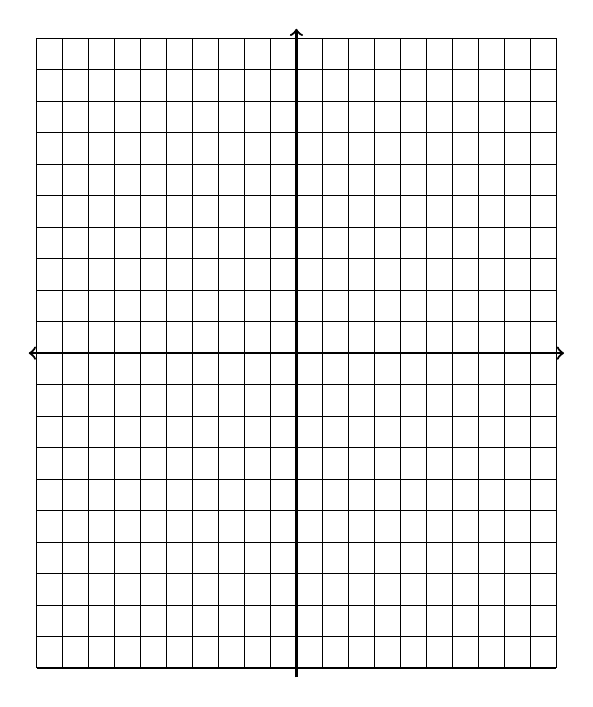
\begin{tikzpicture}[xscale=0.33,yscale=0.04]
	\draw [thick, <->] (-10.3,0) -- (10.3,0);
	\draw [thick, ->] (0,-103) -- (0,103);
	\draw [thin,ystep=10] (-10,-100) grid (10,100);
\end{tikzpicture}

\lab[0104LabSentences] Next, create two algebra sentences for the two symmetries, relating $f(x)$
and $f(-x)$.

\vspace{2cm}

\lab[0104LabBeauty] Do an image search on the internet for ``natural symmetry''.  
Classify what you find as odd, or
even, or rotational.  Taking odd and rotational together and contrasting them with even, 
which kind(s) do you see as more \textit{human} than the other?  Why do you think that is?


\vspace{5cm}
\lab[0104LabPoint] Describe what you think the point of this problem set is, 
using technical vocabulary in complete sentences.
\end{exercises}
\end{multicols*}
